\chapter{Method}
\label{ch:method}

\section*{Literature review}
I reviewed previous work, focusing on two areas. I explored already available
methods for creating animations from sketches by performing skeleton
classification and reviewed previous work dealing with the classification of
sketched objects.

\section*{Related work}
\textcite{eitz2012hdhso} collected a dataset of 20,000 sketches and divided them
into 250 categories of 80 images each. Humans recognized on average 73.1\% of 
these sketches correctly. This dataset is used in my work to train and validate
the classifier to choose which animation is the most appropriate to show.

\textcite{10.1145/3469877.3490565} proposes a pipeline to create rigged and
animated characters from a single image. Their solution aims for a holistic
approach, requiring no user intervention, to assist non-professional users in
creating animated characters. The proposed pipeline performs contour extraction
with salient object detection and extrudes a 3D mesh from geometry generated by
applying constrained Delaunay to the contours. Afterwards, a skeleton is
estimated using a mean curve method and an animation is transferred onto the
skeleton. In our work, we want to follow a similar philosophy of no user
interaction and hope to improve the believability of the animated results by not
only classifying the skeleton type but also the subject class of the input
sketch.

In \textcite{10.1145/3592788} a system for automatically animating drawings of
human figures is introduced. The system comprises of a figure detection step
using Mask R-CNN \Textcite{he2018mask} to extract the figures' bounding box and
utilises a pipeline of quantitisation, morphological closing, dilating,
flood filling and retention of the largest remaining polygon for extracting the
subject's mask. This gave more effective results than using Mask R-CNN for their
usecase. We will investigate both apporaches for our work to decide which one we
want to use for extracting masks for sketeches of quadrupeds. The introduced
pipeline then uses a custom pose estimation model based on a ResNet-50 backbone
to predict the current pose. The result of the pose estimation and masking
process is used to generate a rigged model by using the predicted joint
positions to determine the skeleton and assigning each triangle of the mesh to
the bone, nearest to the triangle's centroid. For animating the pipeline uses
motion captured data of human performers to retarget 3D motion to the 2D result.

\section*{Training classification models}
We used a subset of the dataset provided by \textcite{eitz2012hdhso} and
\textcite{10.1145/2897824.2925954} to train our classification models.
Only the classes "cat" and "dog" were taken as training data for our models. 
To train and evaluate our models we used the scikit-learn library introduced by
\textcite{scikit-learn}.

\subsection*{kNN classifier}
We trained a kNN classifier with the pixel values of the input images. Before
using the values to train the model, we resized the images to a size of 64 times 
64 pixels, and flattened the array to get a feature vector with 12288 entries, 
ranging from 0 to 255 in value. To find the best-performing k, we performed a
grid search with cross-validation on 3 folds leading to k = 5 as the model with 
the highest accuracy at 61.8798\%.

\subsection*{SVM classifier}
We trained an SVM classifier with a total of 1544 labeled images of sketches of
cats and dogs. Before training the model we resized the images to a size of 64
times 64 pixels, and flattened the array to get a feature vector with 4480
entries. The images were imported as grayscale images. The SVM classifier
performed with an accuracy of 53.7578\%.


\subsection*{Neural network classifier}
We created and trained a Neural Network binary classifier using pytorch
\textcite{pytorch}. This is the network's setup:

\begin{python}
    class MyNN(nn.Module):
    def __init__(self):
        super().__init__()
        self.linear_relu_stack = nn.Sequential(
            nn.Linear(in_features=3*128*128,out_features=16*16),
            nn.ReLU(),
            nn.Linear(in_features=16*16,out_features=16*16),
            nn.ReLU(),
            nn.Linear(in_features=16*16,out_features=1)
        )
    def forward(self, x, **kwargs):
        x = x.view(x.size(0), -1)
        logits = self.linear_relu_stack(x)
        return logits
\end{python}

The network was trained on 80\% of a collection of in total 1544 labeled images,
depicting sketches of cats and dogs. The images where resized to a size of
128 times 128 pixels before being fed into the network. Training the network on
80\% of the dataset for 500 epochs with a learning rate of 0.0001, led to the
network performing with a 59.15\% accuracy on the unseen test data.

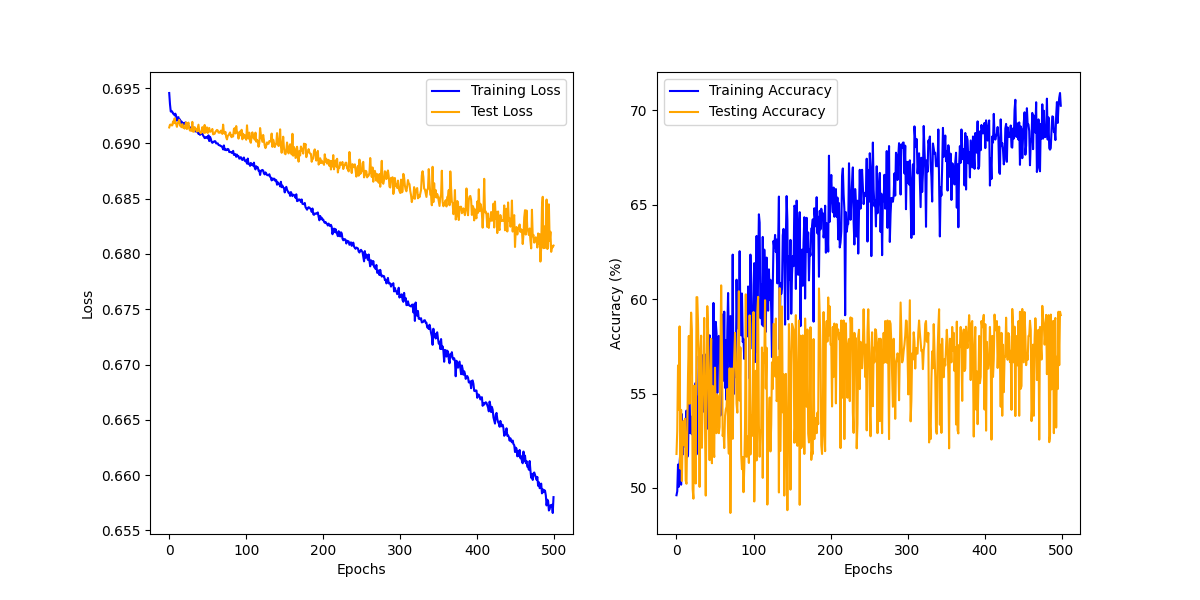
\includegraphics[width=\textwidth]{Figures/NN_classifier_charts.png}

\subsection*{CNN classifier}

We trained a Convolutional Neural Network classifier. This is the network's
setup:

\begin{python}
    class MyCNN(nn.Module):
    def __init__(self):
        super(MyCNN, self).__init__()
        self.conv1 = nn.Conv2d(in_channels=3, out_channels=32,
        kernel_size=3, stride=1,
        padding=1)
        self.conv2 = nn.Conv2d(in_channels=32, out_channels=64,
        kernel_size=3,
        stride=1,
        padding=1)
        self.pool = nn.MaxPool2d(kernel_size=2, stride=2, padding=0)

        self.fc1 = nn.Linear(64 * 32 * 32, 512)
        self.fc2 = nn.Linear(512, 1)

    def forward(self, x):
        x = self.pool(F.relu(self.conv1(x)))
        x = self.pool(F.relu(self.conv2(x)))
        x = x.view(-1, 64 * 32 * 32)
        x = F.relu(self.fc1(x))
        x = self.fc2(x)
        return x
\end{python}

Training the network analogous to the previously mentioned Neural Network
classifier for 500 epochs with a learning rate of 0.0001, yielded an accuracy of
59.15\% on unseen test data.

\includegraphics*[width=\textwidth]{Figures/CNN_classifier_charts.png}

Repeating the setup with a learning rate of 0.001 led to an accuracy of 63.2\%
on unseen test data.

\includegraphics*[width=\textwidth]{Figures/CNN_classifier_lr_001_charts.png}

\subsection*{Enhanced CNN}

We used a slightly more complex CNN architecture adding batch normalization
after each convolutional layer. Also we added an additional Convolution.
Additionally we use a dropout layer before the final fully connected layer.

\begin{python}
    class EnhancedCNN(nn.Module):
        def __init__(self):
            super(EnhancedCNN, self).__init__()

            self.conv1 = nn.Conv2d(in_channels=3, out_channels=32,
             kernel_size=3, stride=1, padding=1)
            self.bn1 = nn.BatchNorm2d(32)
            self.conv2 = nn.Conv2d(in_channels=32, out_channels=32,
             kernel_size=3, stride=1, padding=1)
            self.bn2 = nn.BatchNorm2d(32)
            self.pool1 = nn.MaxPool2d(kernel_size=2, stride=2)

            self.conv3 = nn.Conv2d(in_channels=32, out_channels=64,
            kernel_size=3, stride=1, padding=1)
            self.bn3 = nn.BatchNorm2d(64)
            self.conv4 = nn.Conv2d(in_channels=64, out_channels=64,
            kernel_size=3, stride=1, padding=1)
            self.bn4 = nn.BatchNorm2d(64)
            self.pool2 = nn.MaxPool2d(kernel_size=2, stride=2)

            self.fc1 = nn.Linear(64 * 32 * 32, 512)
            self.dropout1 = nn.Dropout(0.5)
            self.fc2 = nn.Linear(512, 1)

        def forward(self, x):
            x = self.pool1(
                F.relu(
                    self.bn2(
                        self.conv2(F.relu(self.bn1(self.conv1(x))))
                    )
                )
            )

            x = self.pool2(
                F.relu(
                    self.bn4(
                        self.conv4(F.relu(self.bn3(self.conv3(x))))
                    )
                )
            )

            x = x.view(-1, 64 * 32 * 32)

            x = F.relu(self.fc1(x))
            x = self.dropout1(x)
            x = self.fc2(x)
            return x
\end{python}

Training this model with a learning rate of 0.001 for 500 epochs resulted in an
accuracy of 64.79\% on previously unseen test data. It yielded an accuracy of
100\% on the training data. We therefore suspect it to be overfitted.

\includegraphics*[width=\textwidth]{Figures/EnhancedCNN_LR0.001_500.png}

Training the model with a learning rate of 0.0001 for 500 epochs resulted in an
accuracy of 64.07\% on previously unseen test data.

\includegraphics*[width=\textwidth]{Figures/EnhancedCNN_LR0.0001_500Epochs.png}

We introduced 2 additional dropout layers to the network architecture.
The network is described like this:

\begin{python}
    class EnhancedCNNMoreDropout(nn.Module):
    def __init__(self):
        super(EnhancedCNNMoreDropout, self).__init__()

        self.conv1 = nn.Conv2d(in_channels=3, out_channels=32, kernel_size=3, stride=1, padding=1)
        self.bn1 = nn.BatchNorm2d(32)
        self.conv2 = nn.Conv2d(in_channels=32, out_channels=32, kernel_size=3, stride=1, padding=1)
        self.bn2 = nn.BatchNorm2d(32)
        self.pool1 = nn.MaxPool2d(kernel_size=2, stride=2)
        self.dropout1 = nn.Dropout(0.3)

        self.conv3 = nn.Conv2d(in_channels=32, out_channels=64, kernel_size=3, stride=1, padding=1)
        self.bn3 = nn.BatchNorm2d(64)
        self.conv4 = nn.Conv2d(in_channels=64, out_channels=64, kernel_size=3, stride=1, padding=1)
        self.bn4 = nn.BatchNorm2d(64)
        self.pool2 = nn.MaxPool2d(kernel_size=2, stride=2)
        self.dropout2 = nn.Dropout(0.4)

        self.fc1 = nn.Linear(64 * 32 * 32, 512)
        self.dropout3 = nn.Dropout(0.3)
        self.fc2 = nn.Linear(512, 1)

    def forward(self, x):
        x = self.pool1(F.relu(self.bn2(self.conv2(F.relu(self.bn1(self.conv1(x)))))))
        x = self.dropout1(x)

        x = self.pool2(F.relu(self.bn4(self.conv4(F.relu(self.bn3(self.conv3(x)))))))
        x = self.dropout2(x)

        x = x.view(-1, 64 * 32 * 32)

        x = F.relu(self.fc1(x))
        x = self.dropout3(x)
        x = self.fc2(x)
        return x
\end{python}

Introducing a dropout with a value of 0.3 after each convolution block resulted
in a model that achieved 65.43\% on previously unseen test data after being
trained for 500 epochs with a learning rate of 0.0001.

\includegraphics*[width=\textwidth]
{Figures/EnhancedCNNMoreDropoutLR0.0001_500.png}

Setting the dropout to a value of 0.1 resulted in a model that achieved an
accuracy of 58.68\% on previously unseen test data after training for 500 epochs
with a learning rate of 0.0001.

\includegraphics*[width=\textwidth]
{Figures/EnhancedCNNMoreDropout0.1.png}

Setting the dropout to a value of 0.5 resulted in a model that achieved an
accuracy of 67.14\% on previously unseen test data after training for 500 epochs
with a learning rate of 0.0001. The graph led us to believe the model might
benefit from training for a larger amount of epochs.

\includegraphics*[width=\textwidth]
{Figures/EnhancedWithDropoutLR0.0001DO0.5_500.png}

Training with 2000 epochs did not yield an improvement, during our exeriment the
model achieved an accuracy of 59.33\% on previously unseen test data after
training.

\includegraphics*[width=\textwidth]
{Figures/EnhancedCNNWithDropout0.5_2000Epochs.png}



\subsection*{ResNet50 classifier}
We trained a ResNet50 classifier using this pytorch code:

\begin{python}
    class MyResNet50(nn.Module):
    def __init__(self):
        super(MyResNet50, self).__init__()
        self.resnet = models.resnet50(pretrained=True)
        num_features = self.resnet.fc.in_features
        self.resnet.fc = nn.Linear(num_features, 1)

    def forward(self, x):
        x = self.resnet(x)
        return torch.sigmoid(x)
\end{python}

Training the network for 500 epochs with a learning rate of 0.0001 resulted in
an accuracy of 46.46\% on previously unseen test data.

\includegraphics*[width=\textwidth]{Figures/ResNet50_classifier_0001.png}

Training for 500 epochs with a learning rate of 0.001 resulted in an accuracy
of 52.13\% on previously unseen test data.

\includegraphics*[width=\textwidth]{Figures/ResNet50_classifier_LR001_chart.png}

Training the model from scratch by setting pretrained=False, with a learning
rate of 0.001 for 500 epochs resulted in an  accuracy of 49.15\% on previously
unseen test data

\includegraphics*[width=\textwidth]{Figures/ResNet50_untrained_LR001.png}

Training the model from scratch, with a learning rate of 0.001 for 2000 epochs
resulted in an accuracy of 51.64\% on previously unseen test data

\includegraphics*[width=\textwidth]{Figures/ResNet50_untrain_LR001_2000.png}

\section*{Implementing the pipeline}
For this work, we reimplemented the pipeline proposed by
\textcite{korpitsch-2023-sao}, and adapted the code where needed.

\subsection*{Sketchdetection}
To repeat the steps introduced by \textcite{korpitsch-2023-sao} we collected the
dataset provided by \textcite{sarvadevabhatla2017sketchparse}. In
\textcite{smith2023method}, a Mask-R-CNN, as described by \textcite{he2018mask},
is used to detect the bounding boxes of figures drawn by children. 